
\documentclass[a4paper]{article}
\usepackage{graphicx} % Required for \includegraphics command
\usepackage[pages=all, color=black, position={current page.south}, placement=bottom, scale=1, opacity=1, vshift=5mm]{background}
\usepackage[margin=1in]{geometry} % full-width

% AMS Packages
\usepackage{amsmath}
\usepackage{amsthm}
\usepackage{amssymb}

% Unicode
\usepackage[utf8]{inputenc}
\usepackage{hyperref}
\hypersetup{
	unicode,
%	colorlinks,
%	breaklinks,
%	urlcolor=cyan, 
%	linkcolor=blue, 
	pdfauthor={Author One, Author Two, Author Three},
	pdftitle={A simple article template},
	pdfsubject={A simple article template},
	pdfkeywords={article, template, simple},
	pdfproducer={LaTeX},
	pdfcreator={pdflatex}
}

% Vietnamese
%\usepackage{vntex}

% Natbib
\usepackage[sort&compress,numbers,square]{natbib}
\bibliographystyle{mplainnat}

% Theorem, Lemma, etc
\theoremstyle{plain}
\newtheorem{theorem}{Theorem}
\newtheorem{corollary}[theorem]{Corollary}
\newtheorem{lemma}[theorem]{Lemma}
\newtheorem{claim}{Claim}[theorem]
\newtheorem{axiom}[theorem]{Axiom}
\newtheorem{conjecture}[theorem]{Conjecture}
\newtheorem{fact}[theorem]{Fact}
\newtheorem{hypothesis}[theorem]{Hypothesis}
\newtheorem{assumption}[theorem]{Assumption}
\newtheorem{proposition}[theorem]{Proposition}
\newtheorem{criterion}[theorem]{Criterion}
\theoremstyle{definition}
\newtheorem{definition}[theorem]{Definition}
\newtheorem{example}[theorem]{Example}
\newtheorem{remark}[theorem]{Remark}
\newtheorem{problem}[theorem]{Problem}
\newtheorem{principle}[theorem]{Principle}

\usepackage{graphicx, color}
\graphicspath{{fig/}}

%\usepackage[linesnumbered,ruled,vlined,commentsnumbered]{algorithm2e} % use algorithm2e for typesetting algorithms
\usepackage{algorithm, algpseudocode} % use algorithm and algorithmicx for typesetting algorithms
\usepackage{mathrsfs} % for \mathscr command

\usepackage{lipsum}

\renewcommand{\baselinestretch}{1.1} % Change the value to adjust spacing
% Author info
\title{\bfseries \huge Basic Machine Learning approaches for Face Recognition on LFW datset}

\author{\bfseries \Large Gaurav Manish$^1$\and \bfseries \Large Hitesh Singh Parihar$^2$ \and \bfseries \Large Aditya Jaiswal$^3$\and \bfseries \Large Ashutosh Kumar$^4$\and \bfseries \Large Vibhor Saxena $^6$}

\date{ \bfseries \Large
	$^1$Indian Institute Of Technology,Jodhpur \\ \textbf{\{  b22cs079 , b22ee0089 , b22cs025 , b22cs015,c23cs1005\}@iitj.ac.in}\\%
	\texttt
%	\today
}
% Redefining the abstract environment to make the heading bigger
\renewenvironment{abstract}
 {\Large\textbf{Abstract}\vspace{0.5em}\par\noindent\ignorespaces}
 {\par\vspace{0.5em}}
 \usepackage{multirow}
\begin{document}
	\maketitle
	
	\begin  {abstract}
 \fontsize{15}{15}\selectfont 
 In the landscape of computer vision, face recognition stands as a pivotal challenge with far-reaching implications across industries. The ability to automatically identify and authenticate individuals from visual data is not only a technological feat but also a cornerstone for numerous applications, from security systems to personalized user experiences.\vspace{8pt}

This project delves deep into the intricacies of face recognition, focusing on the application of machine learning algorithms to the Labeled Faces in the Wild (LFW) dataset. Our objective is to dissect the effectiveness of various feature extraction techniques and classification algorithms in accurately recognizing faces from diverse and complex datasets.\vspace{8pt}

At the heart of our investigation lies the fundamental problem of face recognition: discerning unique facial characteristics amidst varying lighting conditions, facial expressions, and poses. By tackling this challenge, we aim to unravel the underlying mechanisms that govern the recognition process and pave the way for more robust and reliable face recognition systems.\vspace{8pt}

Throughout our exploration, we have made several significant findings. Firstly, we discovered that feature extraction techniques such as Convolutional Neural Networks (CNN), Local Binary Patterns (LBP), and Histogram of Oriented Gradients (HOG) play a crucial role in capturing distinctive facial features. Moreover, integrating Linear Discriminant Analysis (LDA) with these techniques enhances the discriminative power of the extracted features, leading to improved classification performance.\vspace{8pt}

Our project is structured around these key findings, with each component meticulously designed to explore different facets of the face recognition problem. The report is organized into sections corresponding to each stage of our investigation, including data preprocessing, feature extraction, dimensionality reduction, and classification. Within each section, we present our methodologies, experimental results, and critical insights garnered from our analysis.\vspace{8pt}

By elucidating the intricacies of face recognition algorithms and their performance under various conditions, this report aims to provide a comprehensive understanding of the state-of-the-art techniques in the field. Our findings not only shed light on the challenges inherent in face recognition but also offer valuable insights for researchers and practitioners striving to develop more efficient and reliable face recognition systems.\vspace{8pt}
	
		\noindent\textbf{Keywords:} LFW , CNN , LBP , HOG 
	\end{abstract}

	\tableofcontents
	
	\section{Introduction}
	\label{sec:intro}
  \fontsize{15}{15}\selectfont 
Face recognition is a fundamental task in computer vision with applications ranging from security systems to social media tagging. In this project, we explore various machine learning algorithms for face recognition using the Labeled Faces in the Wild (LFW) dataset. Leveraging the Kaggle API, we access the dataset and preprocess it for feature extraction.\vspace{8pt}

We implement three feature extraction techniques: Convolutional Neural Networks (CNN), Local Binary Patterns (LBP), and Histogram of Oriented Gradients (HOG). Additionally, we integrate Linear Discriminant Analysis (LDA) with these techniques to enhance discriminative power.\vspace{8pt}

Our project consists of six Jupyter Notebooks, each focusing on different combinations of feature extraction and dimensionality reduction techniques. Specifically, we have notebooks for CNN, LBP, and HOG individually, as well as combinations such as CNN with LDA, LBP with LDA, and HOG with LDA.\vspace{8pt}

To evaluate the performance of our models, we employ a variety of classifiers including k-Nearest Neighbors (KNN), Artificial Neural Networks (ANN) using both Scikit-learn and TensorFlow Keras, Random Forest, Support Vector Machines (SVM), Logistic Regression, and Gaussian Naive Bayes. The report is structured to compare the results obtained using different algorithms as well as provide reasons for the obtained results. \vspace{8pt}

Through extensive experimentation and analysis, we compare the accuracy, computational efficiency, and robustness of these algorithms. Our findings provide valuable insights into the effectiveness of different machine learning approaches for face recognition tasks.\vspace{8pt}
	
	\subsection{Citing paper}
	\textbf{Labeled Faces in the Wild (LFW) Dataset:}
 
 \begin{itemize}
\item "Labeled Faces in the Wild: A Database for Studying Face Recognition in Unconstrained Environments" by Gary B. Huang, Manu Ramesh, Tamara Berg, and Erik Learned-Miller. Available at: http://vis-www.cs.umass.edu/lfw/  
\end{itemize}
\textbf{Feature Extraction Techniques:}
\begin{itemize}
\item Convolutional Neural Networks (CNN): Code referenced using the git-hub link provided
\item Local Binary Patterns (LBP): Code referenced using the git-hub link provided
\item Histogram of Oriented Gradients (HOG): Code referenced using the git-hub link provided
\end{itemize}
\textbf{Linear Discriminant Analysis (LDA):}
\begin{itemize}
\item "Pattern Classification" by Richard O. Duda, Peter E. Hart, and David G. Stork.
\end{itemize}
\textbf{Classification Algorithms:}
\begin{itemize}
\item k-Nearest Neighbors (KNN): "Pattern Classification" by Richard O. Duda, Peter E. Hart, and David G. Stork.
\item Artificial Neural Networks (ANN): "Deep Learning" by Ian Goodfellow, Yoshua Bengio, and Aaron Courville.
\item Random Forest: "Random Forests" by Leo Breiman.
\item Support Vector Machines (SVM): "A Tutorial on Support Vector Machines for Pattern Recognition" by Christopher J. C. Burges.
\item Logistic Regression: "The Elements of Statistical Learning" by Trevor Hastie, Robert Tibshirani, and Jerome Friedman.
\item Gaussian Naive Bayes: "The Elements of Statistical Learning" by Trevor Hastie, Robert Tibshirani, and Jerome Friedman.
\end{itemize}
\textbf{Software Libraries:}
\begin{itemize}
\item Scikit-learn: "Scikit-learn: Machine Learning in Python" by Fabian Pedregosa et al.
\item TensorFlow: "TensorFlow: Large-Scale Machine Learning on Heterogeneous Systems" by Martín Abadi et al.
\end{itemize}
	\subsection{Figures}
             \begin{figure}[htbp]
                \centering
                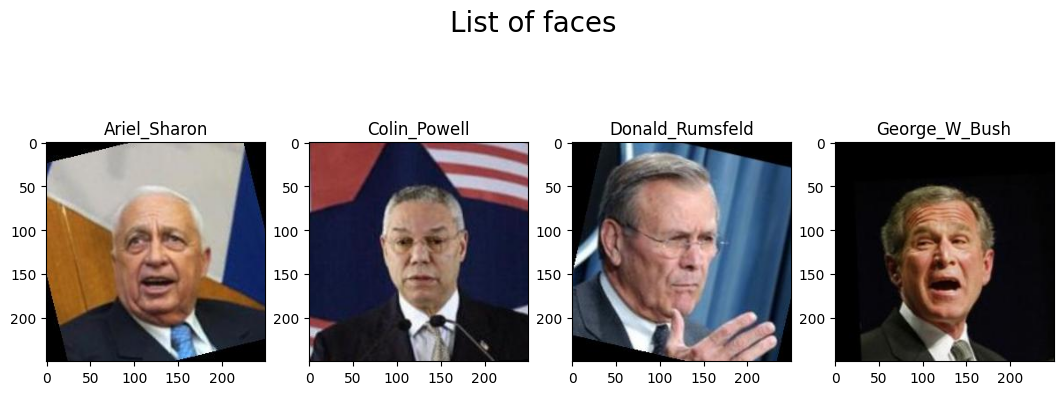
\includegraphics[width=1\textwidth]{allpeople2.png} % Replace "example.jpg" with the filename of your image
                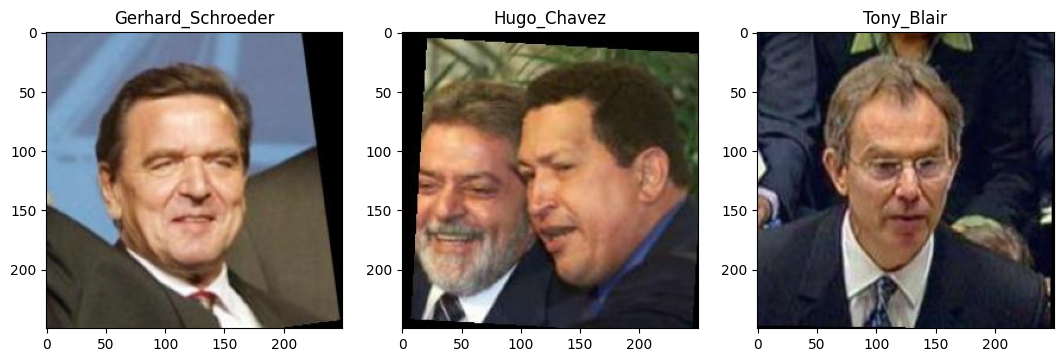
\includegraphics[width=0.9\textwidth]{all_people.png}
                \label{fig:example}
            \end{figure}
            \begin{figure}[htbp]
                \centering
                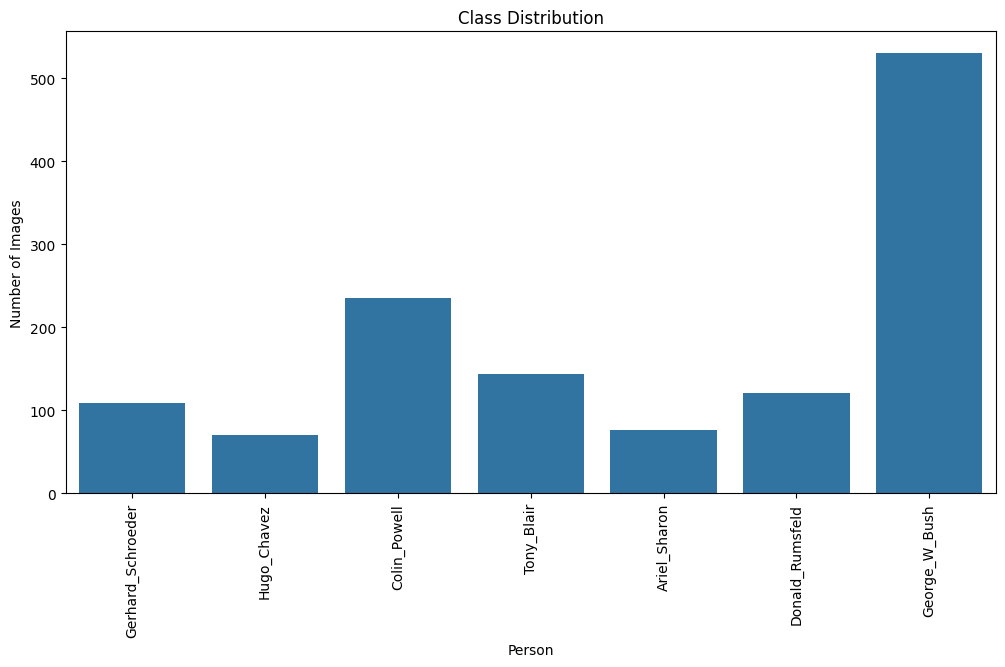
\includegraphics[width=1\textwidth]{countplot.png} % Replace "example.jpg" with the filename of your image
               \caption{VISUALISING COUNTS}
            \end{figure}
            \begin{figure}[htbp]
                \centering
                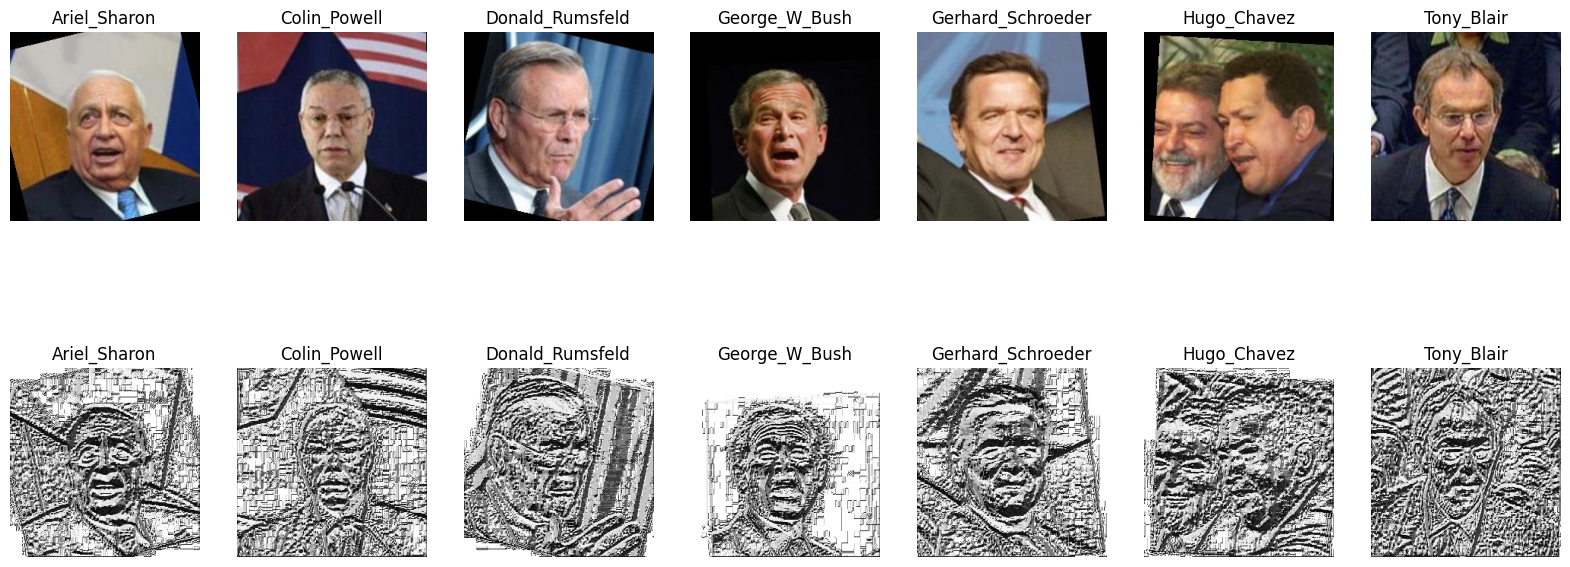
\includegraphics[width=1\textwidth]{lbp.png} % Replace "example.jpg" with the filename of your image
                \caption{VISUALISING LBP IMAGES}
                \label{fig:example}
            \end{figure}
            \begin{figure}[htbp]
                \centering
                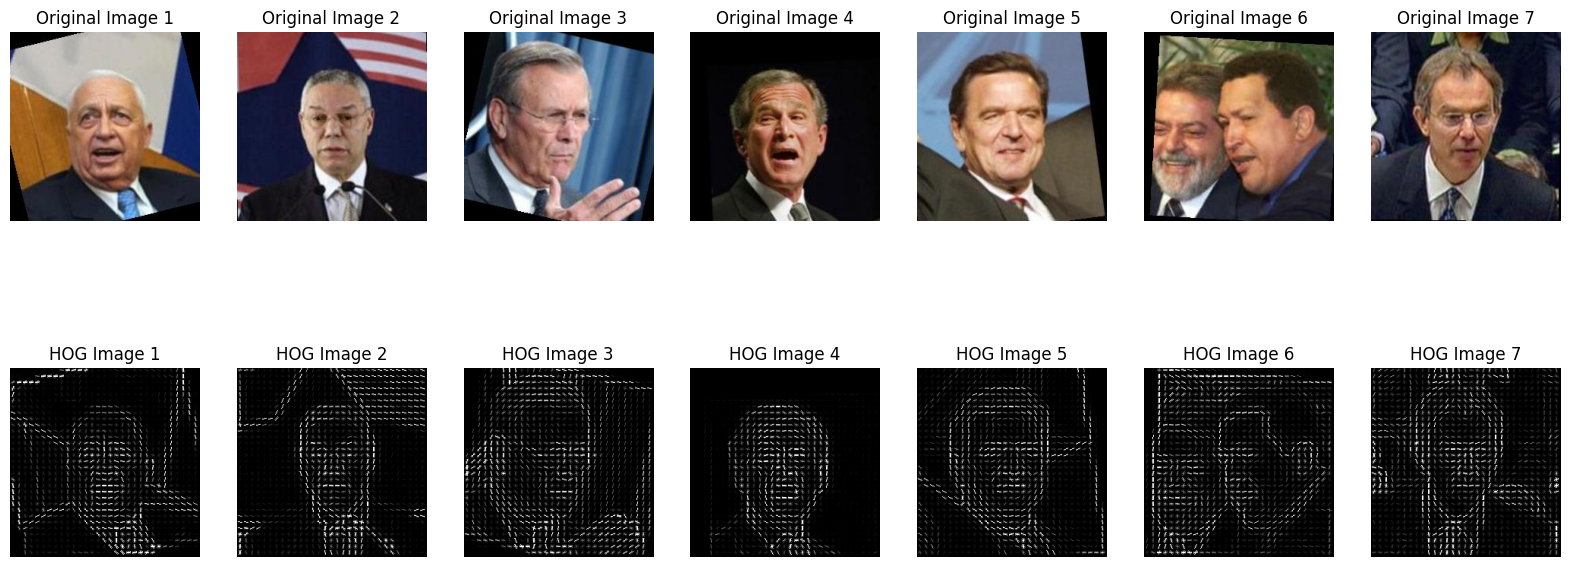
\includegraphics[width=1\textwidth]{hog.png} % Replace "example.jpg" with the filename of your image
                \caption{VISUALISING HOG FEATURES}
                \label{fig:example}
            \end{figure}
            \begin{figure}[htbp]
                \centering
                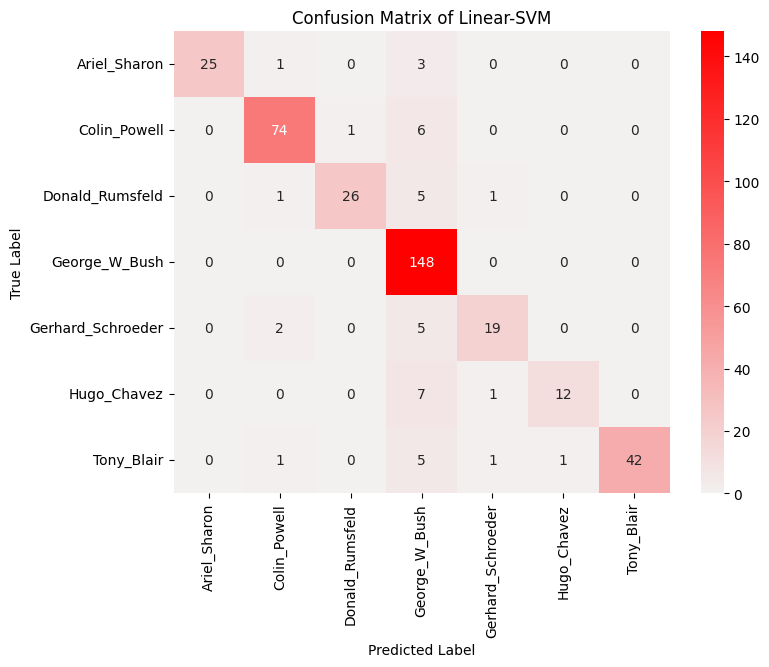
\includegraphics[width=1\textwidth]{LINEARSVM.png} % Replace "example.jpg" with the filename of your image
                \caption{LINEAR SVM ON HOG WITHOUT LDA HAS HIGHEST ACCURACY}
                \label{fig:example}
            \end{figure}
	\newpage
	
	
	\section{Approaches Tried}
	\label{sec:app}
 \textbf{Approach 1: CNN}\vspace{3pt}
  \begin{figure}[htbp]
                \centering
                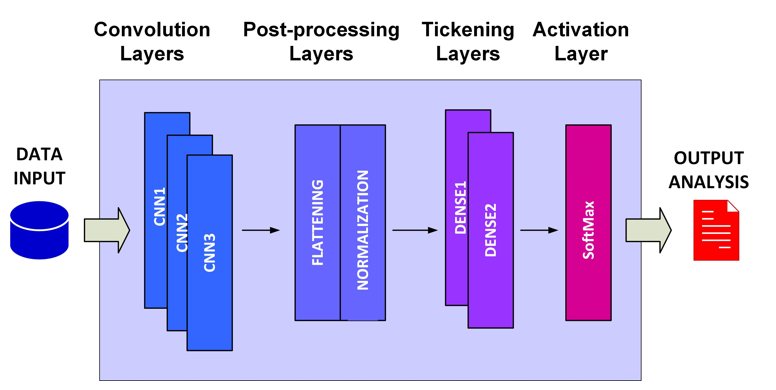
\includegraphics[width=1\textwidth]{normalcnn.png} % Replace "example.jpg" with the filename of your image
                \caption{CNN ARCHITECTURE}
                \label{fig:example}
            \end{figure}
 \begin{itemize}
 \item We apllied CNN to extract 2048 features for each image and then applied basic ML algorithms such as KNN , ANN , Random Forest , Logistic Regression , Gaussian Naive bias.
 \end{itemize}
           
\textbf{Approach 2: LBP}\vspace{3pt}
\begin{figure}[htbp]
                \centering
                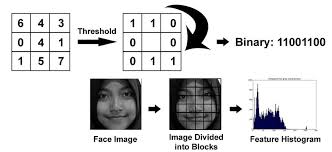
\includegraphics[width=1\textwidth]{lbp-architecture.jpeg} % Replace "example.jpg" with the filename of your image
                \caption{LBP ARCHITECTURE}
                \label{fig:example}
            \end{figure}
 \begin{itemize}
 \item We apllied LBP to extract 256 features for each image and then applied basic ML algorithms such as KNN , ANN , Random Forest , Logistic Regression , Gaussian Naive bias.
 \end{itemize}
 
\textbf{Approach 3: HoG}\vspace{3pt}
 \begin{itemize}
 \item We apllied HoG to extract 70,308 features for each image and then applied basic ML algorithms such as KNN , ANN , Random Forest , Logistic Regression , Gaussian Naive bias.
 \end{itemize}
\begin{figure}[htbp]
                \centering
                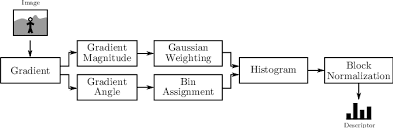
\includegraphics[width=1\textwidth]{HOG-architecture.png} % Replace "example.jpg" with the filename of your image
                \caption{HOG ARCHITECTURE}
                \label{fig:example}
                \end{figure}
\textbf{Approach 4: CNN with LDA}\vspace{3pt}
 \begin{itemize}
 \item We apllied CNN to extract 2048 features for each image , then LDA is used to reduce the dataset into a coordinate space maximizing between class scatter and minimizing within class scatter which resulted in reducing the number of dimensions to 6 as there were 7 labels in our data and finally we applied basic ML algorithms such as KNN , ANN ,Random Forest , Logistic Regression , Gaussian Naive bias on the reduced dataset.
 \end{itemize}
\textbf{Approach 5: LBP with LDA}\vspace{3pt}
 \begin{itemize}
 \item We utilised the Local Binary Patterns (LBP) technique to extract 256 features from each image. Subsequently, Linear Discriminant Analysis (LDA) was employed to reduce the dataset by maximising the scatter between classes and minimising the scatter within classes. This reduction resulted in reducing the number of dimensions to 6, considering the presence of 7 labels in our data. Finally, we applied various fundamental machine learning algorithms, including K-Nearest Neighbours (KNN), Artificial Neural Networks (ANN), Random Forest, Logistic Regression, and Gaussian Naive Bayes, on the reduced dataset.
 \end{itemize}
 \textbf{Approach 6: HoG with LDA}\vspace{3pt}
 \begin{itemize}
 \item First, we used HoG to get 70,308 features for each image. Next, we used LDA to shrink the dataset into a coordinate space that maximised between class scatter and minimised within class scatter. This cut the number of dimensions to 6 because our data had 7 labels. Finally, we used basic machine learning algorithms like KNN, ANN, Random Forest, Logistic Regression, and Gaussian Naive bias on the smaller dataset..
 \end{itemize}
\textbf{The Concepts used in our project and some brief details about them has been provided below:}
	\begin{enumerate}
\item[(A)] \textbf {Convolutional Neural Networks (CNN):}
CNNs are deep learning models specifically designed for processing structured grid data, such as images. They consist of multiple layers of convolutional filters followed by pooling layers, allowing them to automatically learn hierarchical representations of features from raw pixel values.
\item[(B)] \textbf{Local Binary Patterns (LBP):}
LBP is a texture descriptor used for texture classification in images. It encodes local texture patterns by comparing each pixel with its neighboring pixels, resulting in a binary pattern representation. LBP is effective in capturing texture variations in images.
\item[(C)] \textbf{Histogram of Oriented Gradients (HOG):}
HOG is a feature descriptor used for object detection and recognition in images. It computes the distribution of gradient orientations in localized regions of an image. HOG is particularly useful for capturing shape and edge information in images.
\item[(D)] \textbf{Linear Discriminant Analysis (LDA):}
LDA is a dimensionality reduction technique used to find the linear combinations of features that best separate different classes in a dataset. It aims to maximize the between-class scatter while minimizing the within-class scatter, leading to a more discriminative feature space.
\item[(E)] \textbf{k-Nearest Neighbors (KNN):}
KNN is a non-parametric classification algorithm that classifies data points based on the majority vote of their nearest neighbors. It makes predictions by identifying the k nearest data points in the feature space and assigning the class label that is most common among them.
\item[(F)] \textbf{Artificial Neural Networks (ANN):}
ANN is a class of machine learning models inspired by the structure and function of biological neural networks. They consist of interconnected nodes organized in layers, with each node performing a simple computation. ANN can learn complex patterns from data and are widely used for classification tasks.
\begin{figure}[htbp]
                \centering
                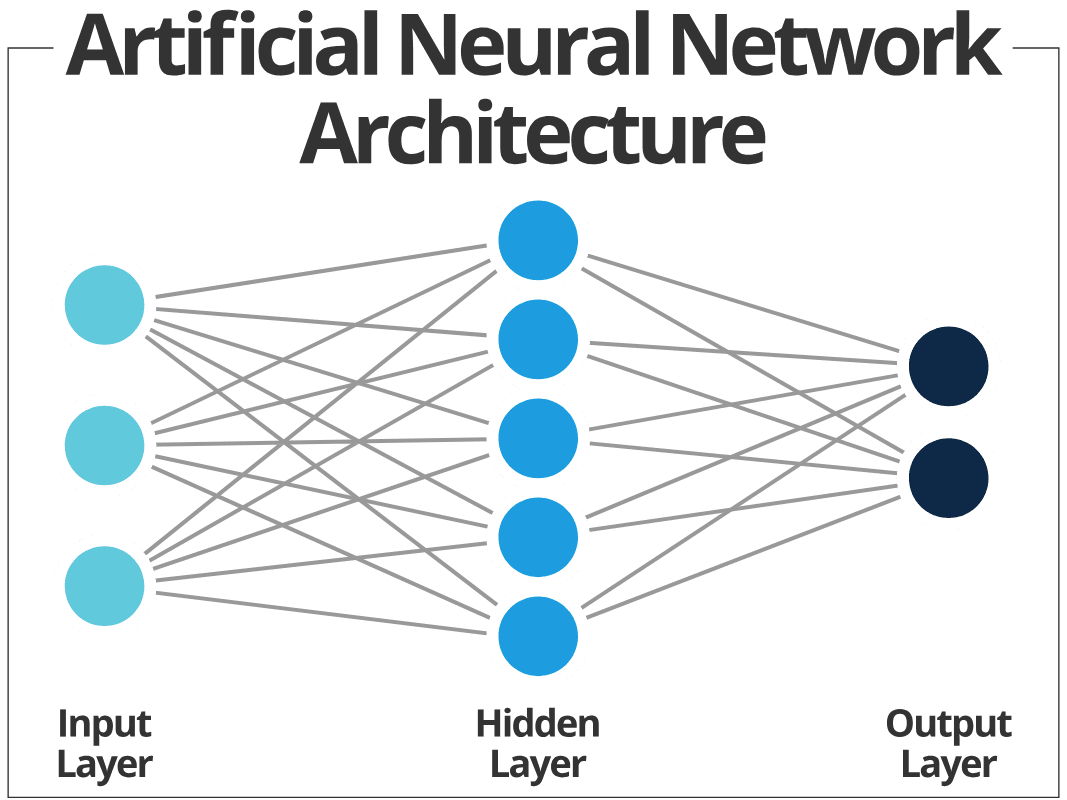
\includegraphics[width=0.8\textwidth,height =0.5\textwidth]{ann-architecture.png} % Replace "example.jpg" with the filename of your image
                \caption{ANN ARCHITECTURE}
                \label{fig:example}
                \end{figure}
\item[(G)] \textbf{Random Forest:}
Random Forest is an ensemble learning method that constructs multiple decision trees during training and outputs the mode of the classes (classification) or the mean prediction (regression) of the individual trees. It is known for its robustness and ability to handle high-dimensional data.
\item[(H)] \textbf{Support Vector Machines (SVM):}
SVM is a supervised learning algorithm used for classification and regression tasks. It constructs a hyperplane in a high-dimensional feature space that separates data points into different classes with the maximum margin. SVM is effective in handling both linear and non-linear classification tasks.
\item[(I)] \textbf{Logistic Regression:}
Logistic Regression is a linear classification algorithm used to model the probability of a binary outcome based on one or more predictor variables. It estimates the parameters of a logistic function that maps input features to the probability of the output class.
\item[(J)] \textbf{Gaussian Naive Bayes:}
Gaussian Naive Bayes is a probabilistic classifier based on Bayes' theorem and the assumption of feature independence. It models the conditional probability of each class given the input features and predicts the class with the highest posterior probability.
 \end{enumerate}
	\newpage

	
	\section{Experiments and Results}
	\label{sec:app}
	The Labeled Faces in the Wild (LFW) dataset is a widely used benchmark dataset in the field of face recognition. It consists of more than 13,000 images of faces collected from the internet, representing over 5,000 different individuals. These images are taken under various conditions, including different lighting, facial expressions, poses, and backgrounds, mimicking real-world scenarios.\vspace{8pt}

In our project we are only loading images of people having atleast 70 images in the dataset to reduce the training time . So in our case the total number of classes are 7.\vspace{8pt} 


\begin{table}[htbp]
\centering
\Large % Set the font size of the table
\caption{Accuracy results for CNN extracted features}
\label{tab:results}
\begin{tabular}{|c|c|c|}
\hline
\textbf{Feature Extraction} & \textbf{Machine Learning Model} & \textbf{Accuracy (\%)} \\ \hline
\multirow{7}{*}{CNN } & k-Nearest Neighbors (KNN) & 56.57 \\ \cline{2-3} 
 & Artificial Neural Networks (ANN) & 79.81 \\ \cline{2-3} 
 & Random Forest & 51.17 \\ \cline{2-3} 
 &  Linear SVM & 76.76 \\ \cline{2-3} 
 & Polynomial SVM & 76 \\ \cline{2-3} 
 & RBF SVM & 78.16 \\ \cline{2-3} 
 & Logistic Regression & 80.28 \\ \cline{2-3} 
 & Gaussian Naive Bayes & 39.67 \\ \cline{2-3}  
 & TensorFlow Keras ANN & 71.83 \\ \hline
% Add more rows for CNN with LDA, LBP, HoG, etc. if needed
\end{tabular}
\end{table}

\begin{table}[htbp]
\centering
\Large
\caption{Accuracy results for CNN with LDA extracted features}
\label{tab:results}
\begin{tabular}{|c|c|c|}
\hline
\textbf{Feature Extraction} & \textbf{Machine Learning Model} & \textbf{Accuracy (\%)} \\ \hline
\multirow{7}{*}{CNN with LDA } & k-Nearest Neighbors (KNN) & 82.86 \\ \cline{2-3} 
 & Artificial Neural Networks (ANN) & 80.7 \\ \cline{2-3} 
 & Random Forest & 79.34 \\ \cline{2-3} 
 &  Linear SVM & 83.09 \\ \cline{2-3} 
 & Polynomial SVM & 80.28 \\ \cline{2-3} 
 & RBF SVM & 84.27 \\ \cline{2-3} 
 & Logistic Regression & 81.92 \\ \cline{2-3} 
 & Gaussian Naive Bayes & 82.86 \\ \cline{2-3}  
 & TensorFlow Keras ANN & 79.57 \\ \hline
% Add more rows for CNN with LDA, LBP, HoG, etc. if needed
\end{tabular}
\end{table}

\begin{table}[htbp]
\centering
\Large
\caption{Accuracy results for LBP extracted feature}
\label{tab:results}
\begin{tabular}{|c|c|c|}
\hline
\textbf{Feature Extraction} & \textbf{Machine Learning Model} & \textbf{Accuracy (\%)} \\ \hline
\multirow{7}{*}{LBP } & k-Nearest Neighbors (KNN) & 37.72 \\ \cline{2-3} 
 & Artificial Neural Networks (ANN) & 23.77 \\ \cline{2-3} 
 & Random Forest & 41.86 \\ \cline{2-3} 
 &  Linear SVM & 43.4 \\ \cline{2-3} 
 & Polynomial SVM & 40 \\ \cline{2-3} 
 & RBF SVM & 38.2 \\ \cline{2-3} 
 & Logistic Regression & 45.2 \\ \cline{2-3} 
 & Gaussian Naive Bayes & 35.65 \\ \cline{2-3}  
 & TensorFlow Keras ANN & 30.49 \\ \hline
% Add more rows for CNN with LDA, LBP, HoG, etc. if needed
\end{tabular}
\end{table}

\begin{table}[htbp]
\centering
\Large
\caption{Accuracy results for LBP with LDA extracted feature}
\label{tab:results}
\begin{tabular}{|c|c|c|}
\hline
\textbf{Feature Extraction} & \textbf{Machine Learning Model} & \textbf{Accuracy (\%)} \\ \hline
\multirow{7}{*}{LBP with LDA} & k-Nearest Neighbors (KNN) & 44.96 \\ \cline{2-3} 
 & Artificial Neural Networks (ANN) & 39.2 \\ \cline{2-3} 
 & Random Forest & 41.6 \\ \cline{2-3} 
 &  Linear SVM & 41 \\ \cline{2-3} 
 & Polynomial SVM & 41.8 \\ \cline{2-3} 
 & RBF SVM & 43.6 \\ \cline{2-3} 
 & Logistic Regression & 79.5 \\ \cline{2-3} 
 & Gaussian Naive Bayes & 79.6 \\ \cline{2-3}  
 & TensorFlow Keras ANN & 42.3 \\ \hline
% Add more rows for CNN with LDA, LBP, HoG, etc. if needed
\end{tabular}
\end{table}

\begin{table}[htbp]
\centering
\Large
\caption{Accuracy results for HoG extracted feature}
\label{tab:results}
\begin{tabular}{|c|c|c|}
\hline
\textbf{Feature Extraction} & \textbf{Machine Learning Model} & \textbf{Accuracy (\%)} \\ \hline
\multirow{7}{*}{HoG} & k-Nearest Neighbors (KNN) & 55.81 \\ \cline{2-3} 
 & Artificial Neural Networks (ANN) & 83.2 \\ \cline{2-3} 
 & Random Forest & 63.56 \\ \cline{2-3} 
 &  Linear SVM & 89 \\ \cline{2-3} 
 & Polynomial SVM & 86 \\ \cline{2-3} 
 & RBF SVM & 70 \\ \cline{2-3} 
 & Logistic Regression & 88.3 \\ \cline{2-3} 
 & Gaussian Naive Bayes & 69.5 \\ \cline{2-3}  
 & TensorFlow Keras ANN & 83.2 \\ \hline
% Add more rows for CNN with LDA, LBP, HoG, etc. if needed
\end{tabular}
\end{table}







\clearpage

\begin{table}[htbp]
\centering
\Large
\caption{Accuracy results for HoG with LDA extracted feature}
\label{tab:results}
\begin{tabular}{|c|c|c|}
\hline
\textbf{Feature Extraction} & \textbf{Machine Learning Model} & \textbf{Accuracy (\%)} \\ \hline
\multirow{7}{*}{Hog with LDA } & k-Nearest Neighbors (KNN) & 79.32 \\ \cline{2-3} 
 & Artificial Neural Networks (ANN) & 82.4 \\ \cline{2-3} 
 & Random Forest & 82.17 \\ \cline{2-3} 
 &  Linear SVM & 82.9 \\ \cline{2-3} 
 & Polynomial SVM & 72.35 \\ \cline{2-3} 
 & RBF SVM & 82.68 \\ \cline{2-3} 
 & Logistic Regression & 86.04 \\ \cline{2-3} 
 & Gaussian Naive Bayes & 82.1 \\ \cline{2-3}  
 & TensorFlow Keras ANN & 87 \\ \hline
% Add more rows for CNN with LDA, LBP, HoG, etc. if needed
\end{tabular}
\end{table}
\textbf{Model with best accuracy:}













	
	
	
	
	\section{Summary}
	\label{sec:app}
 \fontsize{15}{15}\selectfont
	The report presents a comprehensive exploration of machine learning algorithms for face recognition using the Labeled Faces in the Wild (LFW) dataset. The primary focus is on investigating various feature extraction techniques and classification algorithms to achieve accurate and efficient face recognition.\vspace{8pt}

The project begins with data preprocessing, where the LFW dataset is loaded and prepared for feature extraction. Three main feature extraction techniques are explored: Convolutional Neural Networks (CNN), Local Binary Patterns (LBP), and Histogram of Oriented Gradients (HOG). Additionally, Linear Discriminant Analysis (LDA) is integrated with these techniques to enhance feature discriminability and reduce dimensionality.\vspace{8pt}

The report is structured into six distinct sections, corresponding to different combinations of feature extraction and dimensionality reduction methods. Each section includes a detailed methodology, experimental setup, and analysis of results. Various classification algorithms are applied to evaluate the performance of the extracted features, including k-Nearest Neighbors (KNN), Artificial Neural Networks (ANN), Random Forest, Support Vector Machines (SVM), Logistic Regression, and Gaussian Naive Bayes.\vspace{8pt}

Key findings from the experiments reveal the effectiveness of CNN, LBP, and HOG in capturing discriminative facial features. Furthermore, integrating LDA with these techniques significantly improves classification accuracy and robustness. Comparative analysis of classification algorithms highlights their respective strengths and limitations in the context of face recognition tasks.\vspace{8pt}

The report concludes with insights into the most effective combinations of feature extraction and classification algorithms for face recognition. It also discusses potential avenues for future research, including exploring advanced deep learning architectures and incorporating additional contextual information for improved performance.\vspace{8pt}

Overall, the report provides valuable insights into the application of machine learning techniques for face recognition and lays the groundwork for further advancements in this field.\vspace{8pt}
	

	
	\bibliography{refs}
	
	\appendix
	
	\section{Contribution of each member}
	\label{sec:contribution}
	\begin{enumerate}
	\item Gaurav Manish(B22CS079): worked on extraction of features , worked on streamlit, contributed to report
	\item Hitesh Singh Parihar(B22EE089): Helped in applying various models and contributed in preparing report.
 \item Jaiswal Aditya Ranjit(B22CS025):worked on extracting of LBP features , implemented models,  
  \item Ashutosh Kumar(B22CS015): implemented models, Prepared website for the project, worked for the video presentation
  \item Vibhor Saxena (C23CS1005): 
	
	\end{enumerate}
    	
	
\end{document}
